\documentclass{article}
\usepackage[utf8]{inputenc}
\usepackage{amsmath, amssymb, tikz, graphics, biblatex, geometry, float}
\setlength{\parskip}{1em}
\setlength{\parindent}{0em}
\usepackage{enumerate}
\DeclareMathOperator{\Cov}{Cov}
\DeclareMathOperator{\Var}{Var}

\usepackage{pgf,tikz,pgfplots}
\pgfplotsset{compat=1.15}
\usepackage{mathrsfs}
\usetikzlibrary{arrows}
\definecolor{xdxdff}{rgb}{0.49019607843137253,0.49019607843137253,1}
\definecolor{zzttqq}{rgb}{0.6,0.2,0}
\definecolor{uuuuuu}{rgb}{0.26666666666666666,0.26666666666666666,0.26666666666666666}
\definecolor{ffqqtt}{rgb}{1,0,0.2}

\newcommand{\grstep}[2][\relax]{%
   \ensuremath{\mathrel{
       {\mathop{\longrightarrow}\limits^{#2\mathstrut}_{
                                     \begin{subarray}{l} #1 \end{subarray}}}}}}
\newcommand{\swap}{\leftrightarrow}
\usepackage[colorlinks=true,linkcolor=blue, citecolor=blue, allcolors=blue ]{hyperref}
\urlstyle{tt}

\title{MA2216 19/20 Sem 2} 
% Should we publish the paper on the website as well?
\author{Written by: Yip Jung Hon, Audited by: Chong Jing Quan}
\begin{document}
\maketitle
\subsection*{Question 1}
A 5-digit number is formed such that each digit is one of the nine integers 1,2...9. Each integer can be used any number of times.
\begin{enumerate}[i)]
  \item How many 5-digit numbers can be formed?
  
  $9^5 = 59049$.
  \item How many 5-digit numbers can be formed such that no three consecutive digits are the same? 
  
 Consider numbers with 3 or more consecutive digits first. To have 3 consecutive digits, say your repeated digit is r. You can have rrrxx, xrrrx or xxrrr. For rrrxx, choose one number to be r. The x next to the r has 8 choices for 3 consecutive digits. The x 2 steps away from the last r has 9 chocies. xxrrr has a similar reasoning. For xrrrx, both x's are beside the 3 r's, meaning that for each x, there's a total of 8 choices. In total, for 3 consecutive digits, we have: $2*9*8*9 + 9*8*8$.
 
 For numbers with 4 consecutive digits, we can either have rrrrx or xrrrr. Pick one of 9 numbers to be r, then x can take on 8 numbers. Numbers with 4 consecutive digits: $2*8*9$.
 
 Numbers with 5 consecutive digits = 9.
  
  Numbers with 3 consecutive digits = $2*9*8*9 + 9*8*8 + 2*8*9 + 9 = 2025$.
  
  Taking complements, $59049-2025=57024$.
\end{enumerate}

\subsection*{Question 2}
The system contains 4 gates and water flows from $A$ to $B$. The gates work independently and the probability that a gate is open is $p$.
\begin{figure}[H]
    \centering
    \includegraphics[scale=0.15]{probability_gates.png}
\end{figure}
\begin{enumerate}[i)]
 \item What is the probability that water is able to flow from $A$ to $B$?
 
 For water to flow, $1$ must be open. Either 2 must be open or both 3 \& 4 must be open. However, $p+p^2 $ double counts the event where gates 1,2,3 are open. We have to exclude that event. 
 \begin{align*}
     P(A \text{ flows to } B) = p * [p + p^2 - p^3] = p^2(p+1-p^2)
 \end{align*}
 \item What is the conditional probability that gate 2 is open given that water is able to flow from $A$ to $B$?
 
 $P(\text{gate 2 open} \cap \text{water flows from $A$ to $B$}) = p^2$. There is a $p$ chance of gate 1 being open, and a $p$ chance of gate 2 being open. Whether gate 3 or 4 is open or closed is of no concern. 
 $P(\text{gate 2 open} \mid \text{water flows from $A$ to $B$}) = p^2/p^2(p+1-p^2) = 1/(p+1-p^2)$.
\end{enumerate}

\subsection*{Question 3}
The probability density funtion of $X$ is
\[ f(x)=\begin{cases} 
      \frac{x}{100}+\frac{1}{10} & -5<x<5 \\
      0 & \text{otherwise}
   \end{cases}
\]
\begin{enumerate}[i)]
    \item Put $Y=X^2$. Find the PDF of $X^2$. State clearly the range of $Y$ for which there is positive density.
    
    Let's find the CDF of $Y$ first. 
    \begin{align*}
        F_Y(y) &= P(Y \leq y)  \\
        &= P(X^2 \leq y) \\
        &= P(-\sqrt{y} \leq x \leq \sqrt{y}) \\
        &= \int_{-\sqrt{y}}^{\sqrt{y}} \frac{x}{100} + \frac{1}{10} dx \\
        &= \left.\frac{x^2}{200} + \frac{x}{10} \right \vert ^{\sqrt{y}}_{-\sqrt{y}} \\
        &=\frac{\sqrt{y}}{5}
        \end{align*}
    Since the PDF is defined to the derivative of the CDF, $f_Y(y) = F'_Y(y) = \frac{d}{dy} \frac{\sqrt{y}}{5} = \frac{1}{10\sqrt{y}}$, and it has a positive density on $0 < y < 25$.

    \item Let $Z$ be the largest integer less than or equal to $X$. Find the PMF of $Z$. State clearly all the values that can be assumed by $Z$ with positive probabilities. 
    
    $Z \in \{-5, -4, -3, -2, -1, 0,1,2,3,4\}$
    \begin{align*}
        P(Z=z)&= P(z < X < z+1) \\
        &= \int_z^{z+1} \frac{x}{100} + \frac{1}{10} dx \\
        &= \left. \frac{x^2}{200} + \frac{x}{10} \right \vert^{z+1}_z \\
        &= \frac{2z+21}{200}.
    \end{align*}
\end{enumerate}

\subsection*{Question 4}
The joint PDF for $X$ and $Y$ is
\[ f(x,y)=\begin{cases} 
      3x & \text{if } x>0, y<2, y>2x \\
      0 & \text{otherwise}
   \end{cases}
\]
\begin{enumerate}[i)]
    \item Find the PDF of $X$. The range for which the PDF is positive must be clearly specified.
    
    \begin{figure}[H]
        \centering
        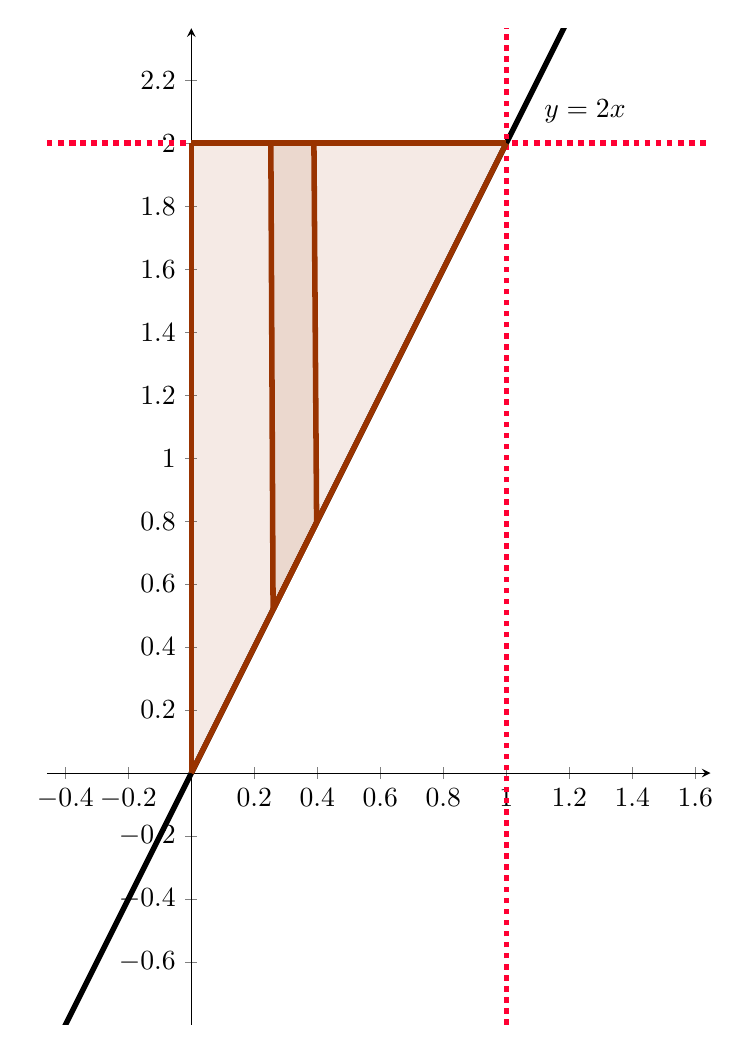
\begin{tikzpicture}
            \begin{axis}[
                    x=4cm,y=4cm,
                    axis lines=middle,
                    xmin=-0.45848617250727247,
                    xmax=1.6484805444488442,
                    ymin=-0.7995518008538336,
                    ymax=2.364851042139802,
                    xtick={-0.4,-0.2,...,1.6},
                    ytick={-0.6000000000000001,-0.4000000000000001,...,2.2},]
                    \clip(-0.45848617250727247,-0.7995518008538336) rectangle (1.6484805444488442,2.364851042139802);
                    \fill[line width=2pt,color=zzttqq,fill=zzttqq,fill opacity=0.10000000149011612] (0,2) -- (1,2) -- (0,0) -- cycle;
                    \fill[line width=2pt,color=zzttqq,fill=zzttqq,fill opacity=0.10000000149011612] (0.2524776280470785,2) -- (0.25958929797838126,0.5191785959567625) -- (0.39778346714159685,0.7955669342831937) -- (0.38925981114800523,2) -- cycle;
                    \draw [line width=2pt,domain=-0.45848617250727247:1.6484805444488442] plot(\x,{(-0--2*\x)/1});
                    \draw [line width=2pt,dotted,color=ffqqtt,domain=-0.45848617250727247:1.6484805444488442] plot(\x,{(--2-0*\x)/1});
                    \draw [line width=2pt,dotted,color=ffqqtt] (1,-0.7995518008538336) -- (1,2.364851042139802);
                    \draw [line width=2pt,color=zzttqq] (0,2)-- (1,2);
                    \draw [line width=2pt,color=zzttqq] (1,2)-- (0,0);
                    \draw [line width=2pt,color=zzttqq] (0,0)-- (0,2);
                    \draw [line width=2pt,color=zzttqq] (0.2524776280470785,2)-- (0.25958929797838126,0.5191785959567625);
                    \draw [line width=2pt,color=zzttqq] (0.25958929797838126,0.5191785959567625)-- (0.39778346714159685,0.7955669342831937);
                    \draw [line width=2pt,color=zzttqq] (0.39778346714159685,0.7955669342831937)-- (0.38925981114800523,2);
                    \draw [line width=2pt,color=zzttqq] (0.38925981114800523,2)-- (0.2524776280470785,2);
                    \begin{scriptsize}
                    \draw[color=black] (1.25 ,2.1) node {$y=2x$};
                    \end{scriptsize}
                    \end{axis}
        \end{tikzpicture}
    \end{figure}

The shaded region is the one we want. Integrating along the $y$-axis, our integral runs from $2$ to $2x$, as seen in the vertical bar in the image above. So,
\begin{align*}
    f_X(x) &= \int_{2x}^2 f_{X, Y} (x,y) dy \\
    &= \int_{2x}^2 3x \ dy \\
    &= 6x -6x^2
\end{align*}
which has a positive density on $0<x<1$.
\item Find the conditional PDF $f_{X \mid Y} (x| y)$. Are $X$ and $Y$ independent?

\begin{align*}
    f_Y(y) &= \int^{\frac{y}{2}}_0 f_{X, Y} (x,y) dx \\
    &=\int^{\frac{y}{2}}_0 3x \ dx \\
    &= \frac{3y^2}{8} 
\end{align*}
which has a positive density on $0<y<2$.
\begin{align*}
    f_{X \mid Y=y}(x) &= \frac{f_{X, Y} (x,y)}{f_Y(y)} \\
    &= \frac{3x}{\frac{3y^2}{8}}\\
    &=\frac{8x}{y^2}.
\end{align*}
$X$ and $Y$ are not independent since $f_Y(y) \times f_X(x) \neq  f_{X, Y} (x,y)$.
\item Find $\Cov(X,Y)$ and explain why it is positive.
\begin{equation}
    E(XY) = \int_0^2 E(Xy \mid Y=y) f_Y(y) dy = \int_0^2 y E(X \mid Y=y) f_Y(y) dy \label{eq1}
\end{equation}
\begin{align*}
    E(X \mid Y=y) &= \int_0^{\frac{y}{2}} xf_{X \mid Y=y}(x) dx \\
    &= \int_0^{\frac{y}{2}} x\frac{8x}{y^2} dx \\
    &= \left.\frac{8x^3}{3y^2}\right|_0^{\frac{y}{2}} \\
    &= \frac{y}{3}
\end{align*}
Subbing back into (\ref{eq1}),
\begin{align*}
    E(XY) &= \int_0^2 y \frac{y}{3} \frac{3y^2}{8} dx \\
    &= \int_0^2 \frac{y^4}{8} dy \\
    &= \frac{4}{5}.
\end{align*}
Further, $E(X) = \int_0^1 x(6x-6x^2) dx = \frac{1}{2}$, and $E(Y)= \int_0^2 y \frac{3y^2}{8} dy = \frac{3}{2}$.
\begin{equation*}
    \Cov(X,Y) = E(XY)-E(X)E(Y) = \frac{4}{5} - \frac{1}{2} \times \frac{3}{2} = \frac{1}{20}.
\end{equation*}
$\Cov(X,Y)$ is positive because when the random variable takes on a larger number, the probability that $Y$ would take on a larger number increases as well, since one must have $y>2x$.
\end{enumerate}

\subsection*{Question 5}
Two points are selected randomly on a line of length 1. Put $X$ as the smaller of the two points and $Y$ as the larger of the two points. 
\begin{enumerate}[i)]
\item Find the joint probability density function of $X$ and $Y$.

Let $U$ and $V$ be random variables denoting which values the first and second points land on respectively. From independence,
\begin{equation*}
    f_{U,V}(u,v)=1 \text{  for } 0 \leq u,v \leq 1.
\end{equation*}
Put $Y=\max(U,V)$, $X=\min(U,V)$. Fix some $h>0$. Note that:
\begin{equation*}
    P(x < X < x+h, y< Y<y+h) = P(x < U < x+h, y< V<y+h) +P(y < U < y+h, x< V<x+h)
\end{equation*}
This is because for $X$ to take on a range of values, say in $(x, x+h)$, and $Y$ to be in $(y, y+h)$, either $U$ must be in $(x, x+h)$ and $V$ must be in $(y, y+h)$, or $V$ must be in $(x, x+h)$ and $U$ must be in $(y, y+h)$. Taking $\lim_{h \to 0}$,
\begin{equation*}
    f_{X,Y}(x,y) = P(x < X < x+h, y< Y<y+h) = f_{U,V}(x,y) + f_{U,V}(y,x) = 2.
\end{equation*}
So $f_{X,Y}(x,y) =2$ for $0\leq x \leq y \leq 1$.
\item What is the expected length of $E(Y-X)$ \footnote{This is a famous problem. Generalisations include the expected distance between two points chosen randomly on the circumference of a circle and the expected distance between two random points in a square and circle. }?

\begin{equation*}
    f_Y(y) = \int_0^y f_{X,Y}(x,y) dx = \int_0^y 2 dx = 2y.
\end{equation*}
\begin{equation*}
    f_X(y) = \int_x^1 f_{X,Y}(x,y) dx = \int_0^y 2 dx = 2-2x.
\end{equation*}
\begin{equation*}
    E(Y) = \int_0^1 2y^2 dy = \frac{2}{3}
\end{equation*}
\begin{equation*}
    E(X) = \int_0^1 x(2-2x) dx = \frac{1}{3}
\end{equation*}
Now, from linearity of expectation, 
\begin{equation*}
    E(Y-X)=E(Y)-E(X) = \frac{1}{3}.
\end{equation*}
\end{enumerate}

\subsection*{Question 6}
Jar A contains 2 tags numbered 1 and 2 respectively. Jar B also contains 2 tags numbered 1 and 2 respectively. Jar C contains 3 tags numbered 1,2 and 3 respectively. We select one tag at random from $A$. Record the number as $X_1$. We then select randomly $X_1$tags from $B$ with replacement. Let $X_2$ be the total number on the tags drawn from B. We finally select $X_2$ tags randomly from $C$ with replacement. Let $X_3$ be the total number on the tags drawn from $C$. Find $E(X_3)$.

By the LOTP, we may break $E(X_3)$ into
\begin{align*}
    E(X_3) &= E(X_3 \mid X_2 = 1) P(X_2=1) + E(X_3 \mid X_2 = 2) P(X_2=2) \\
    &+E(X_3 \mid X_2 = 3) P(X_2=3) +E(X_3 \mid X_2 = 4) P(X_2=4)  
\end{align*}
\begin{align*}
    P(X_2=1) &\iff \text{you get 1 draw and you draw only 1 from A} \\
    &= \frac{1}{2} \times \frac{1}{2} = \frac{1}{4}\\
    P(X_2=2) &\iff \text{you get 1 draw and you draw 2, or you get 2 draws and draw both 1's} \\
    &= \frac{1}{2} \times \frac{1}{2} + \frac{1}{2} \times \frac{1}{4} \\
    &= \frac{3}{8} \\
    P(X_2=3) &\iff \text{you get 2 draws and you draw 2 and 1, or 1 then 2} \\
    &= \frac{1}{2} \times \left(\frac{1}{4} + \frac{1}{4} \right) = \frac{1}{4} \\
    P(X_2=4) &\iff \text{you get 2 draws and you draw both 2's} \\
    &= \frac{1}{2} \times \frac{1}{4} = \frac{1}{8}
\end{align*}
Let's say you are only allowed to draw once from C. What is the expected value of that draw? It is,
\begin{equation*}
    E(X_3 \mid X_2 = 1) = \frac{1}{3} \times 1 + \frac{1}{3} \times 2 \times \frac{1}{3} \times 3 = 2 
\end{equation*}
However, the draws are \textbf{with replacement}, meaning that for each draw, one returns to the urn with the values, meaning the expected value for each draw does not change. So $E(X_3 \mid X_2 = k)=2k$.
\begin{equation*}
    E(X_3) = 2 \times \frac{1}{4} + 4 \times \frac{3}{8} + 6 \times \frac{1}{4} + 8 \times \frac{1}{8} = \frac{9}{2}.
\end{equation*}

\subsection*{Question 7}
Let $X$ and $Y$ be independent standard normal variables. Calculate the conditional expectation $E(X^3 - Y^3 \mid X-Y = 1)$. (Hint: $X+Y$ and $X-Y$ are independent. You may assume this without proof.

\begin{align*}
    E(X^3 - Y^3 \mid X-Y=1) &= E((X-Y)(X^2+ XY + Y^2 \mid X-Y=1) \\
    &= E(X^2+ XY + Y^2 \mid X-Y=1) 
\intertext{Sub $X=1+Y$.}
    &= E((1+Y)^2+ (1+Y)Y + Y^2 \mid X-Y=1)  \\
    &= E(1+3Y+Y^2 \mid X-Y=1)
\end{align*}
Put $X-Y=U$, hence $U \sim N(0,2)$. So $f_U(u)= \frac{1}{\sqrt{2\pi}\sqrt{2}}e^{-\frac{x^2}{4}}=\frac{1}{2\sqrt{\pi}}e^{-\frac{x^2}{4}}$.
\begin{align*}
    f_{Y \mid U=1}(y) &= \frac{f_{Y, U}(y,1)}{f_U(1)} \\
    &= \frac{f_{X,Y}(1+y,y)}{f_U(1)} \\
\intertext{From independence,}
    &= \frac{f_{X}(1+y) \times f_Y(y)}{f_U(1)}\\
    &= \frac{\frac{1}{\sqrt{2\pi}}e^{-\frac{(y+1)^2}{2}}\frac{1}{\sqrt{2\pi}}e^{-\frac{(y)^2}{2}}}{\frac{1}{2\sqrt{\pi}}e^{-\frac{x^2}{4}}} \\
    &= \frac{1}{\sqrt{\pi}} \exp\left\{-\left(\frac{(y+1)^2}{2}+\frac{y^2}{2}-\frac{1}{4}\right)\right\} \\
    &= \frac{1}{\sqrt{\pi}} \exp \left\{ -\left(y^2+y+\frac{1}{4} \right)\right\} \\
    &= \frac{1}{\sqrt{\pi}} \exp \left\{ -\left(y+\frac{1}{2} \right)^2\right\}
\end{align*}
This means that $f_{Y \mid U=1} \sim N(-\frac{1}{2}, \frac{1}{2})$ \footnote{It is known that the distribution is uniquely specified by the CDF, PDF or MGF. The proof, however, is not easy.}.
The moment generating function of a normal distribution of mean $\mu$ and variance $\sigma^2$ is:
\begin{equation*}
    M(t) = \exp\left\{t\mu+\frac{1}{2}\sigma^2 t^2\right\} \footnote{This is also why odd moments of a \textbf{standard normal distribution} is 0.}
\end{equation*}
We get that,
\begin{align*}
    E(X) &= M'(0) = \mu = -\frac{1}{2} \\
    E(X^2) &= M''(0) = \sigma^2 + \mu^2 = \left(-\frac{1}{2} \right)^2 + \frac{1}{2} = \frac{3}{4}.
\end{align*}
Lastly, $$E(1+3Y+3Y^2 \mid X-Y=1) = 1+3\left(-\frac{1}{2} \right) + 3 \left( \frac{3}{4}\right) =\frac{7}{4}$$.

\subsubsection*{Another way}
Note that we may write $E(X^3 - Y^3 \mid X-Y = 1)$ as \begin{align*}
    E((X^2 + XY + Y^2 \mid X-Y = 1) &= E(X+Y)^2 - XY \mid X-Y = 1) \\
    &= E\left((X+Y)^2 - \left(\frac{1}{4}(X+Y)^2 - \frac{1}{4}(X-Y)^2 \right)\mid X-Y = 1\right) \\
    &= E\left(\frac{3}{4}(X+Y)^2 + \frac{1}{4}(X-Y)^2 \mid X-Y = 1\right) \\
\end{align*}
We know $X+Y \sim N(0,2)$. You can use MGF's to deduce that $E((X+Y)^2) = \mu^2 + \sigma^2 = 2$, or you can use $\Var(X)=E(X^2) - [E(X)]^2$. 
\begin{align*}
    E\left(\frac{3}{4}(X+Y)^2 + \frac{1}{4}(X-Y)^2 \mid X-Y = 1\right) &= \frac{3}{4} (2)  + \frac{1}{4} (1) \\
    &= \frac{7}{4}.
\end{align*}
\end{document}